%%=============================================================================
%% Methodologie
%%=============================================================================

\chapter{\IfLanguageName{dutch}{Methodologie}{Methodology}}%
\label{ch:methodologie}


%% TODO: Hoe ben je te werk gegaan? Verdeel je onderzoek in grote fasen, en
%% licht in elke fase toe welke stappen je gevolgd hebt. Verantwoord waarom je
%% op deze manier te werk gegaan bent. Je moet kunnen aantonen dat je de best
%% mogelijke manier toegepast hebt om een antwoord te vinden op de
%% onderzoeksvraag.

Nu toegelicht is wat een low-code development platform precies is en hoe het werkt, kan er worden overgaan tot de vergelijkende studie zelf. In dit hoofdstuk wordt de methodologie van het onderzoek beschreven en uitgelegd. Dit is deels een vervolgstuk op de technologieën die in de literatuurstudie besproken werden. Eerst en vooral komt de requirementsanalyse aan bod, waaruit de potentiële kandidaten voor de vergelijkende studie bekomen worden. Daarna wordt een use case opgesteld, die dan in het volgende hoofdstuk zal uitgebouwd worden in Podio en de verschillende alternatieven om vervolgens vergelijkingen te maken. Ten slotte wordt een set van criteria opgesteld die tijdens het onderzoek zal gebruikt worden om de alternatieven te vergelijken met Podio. \\

Omdat Quivvy Solutions het belangrijk vindt up-to-date te blijven over diverse low-code platformen, heeft het bedrijf reeds onderzoek gedaan naar een potentieel alternatief. Om die redenen is één van de kandidaten, Airtable, al gekozen uit de longlist van kandidaten. Dit is een van de platformen waar het bedrijf veel interesse in heeft en graag zou willen onderzoeken. Desondanks het feit dat het platform al geselecteerd is, zullen na de requirementsanalyse de verschillende vereisten voor Airtable toch doorgenomen worden. Dit om aan te tonen dat het een volwaardige kandidaat is voor het onderzoek. \\


\section{Requirementsanalyse}
\label{sec:requirementsanalyse}

De requirements voor een goed alternatief werden opgesteld aan de hand van de noden van Quivvy Solutions. Zij ontwikkelen low-code oplossingen voor kleine tot middelgrote bedrijven en gebruiken daarvoor voornamelijk Podio. De platformen moeten dus ten minste over de basisfunctionaliteiten van Podio beschikken. Bovendien moet er ook worden nagegaan of de alternatieven een goede toekomst hebben. Uiteindelijk werden de nodige vereisten verder opgedeeld in functionele en niet-functionele vereisten. \\

\textbf{Functionele vereisten:}

\begin{itemize}
    \item De datastructuur moet bestaan uit een enkele database die zich als \textbf{'Single source of truth'} voordoet. Met andere woorden, het platform moet voor een applicatie een enkele database voorzien zodat alle data slechts op één plek wordt opgeslagen.
    \item Het platform moet over een bepaald minimum aan \textbf{flexibiliteit} bezitten. Dit betekent het zich niet mag focussen op specifieke use cases, maar dat het gebruikt kan worden voor elke context. Indien iets toch niet mogelijk is, moeten er workarounds of extensies aanwezig zijn die dit probleem verhelpen.
    \item Het platform moet in staat zijn om zaken zoals \textbf{workflows te automatiseren}.
    \item Het platform moet over een \textbf{eigen API} bezitten.
\end{itemize}

\textbf{Niet-functionele vereisten:} 

\begin{itemize}
    \item Het platform moet \textbf{low-code/no-code} zijn.
    \item Het platform moet een stevige \textbf{gebruikersbasis} hebben. Dit betekent dat het ten minste door ongeveer 250.000 gebruikers en 3000 bedrijven in gebruik moet zijn.
    \item Het platform moet \textbf{stabiel} zijn. Dit betekent dat het geen frequente storingen ondervindt en dat het zich beperkt tot maximaal twee incidenten per maand.
    \item Het platform moet \textbf{futureproof} zijn. Dit betekent dat het platform zeer sterk aan het groeien moet zijn. Hierbij wordt gekeken naar het aantal werknemers, de winst en de opgehaalde financiering op jaarbasis.
\end{itemize}


\section{Longlist}
\label{sec:long_list}

Na het definiëren van de requirements kan een longlist van potentiële alternatieven worden opgesteld, deze lijst is terug te vinden in Tabel \ref{tab:Tabel 3}. Verder wordt er ook steeds aangeduid of het platform no-code, low-code of beide is. \\

\begin{table}[h]
    \centering
    \caption{\label{tab:Tabel 3} Lijst met Podio alternatieven die onderzocht kunnen worden \autocite{Tasmia2022}.}
    \begin{tabular}{ | p{5cm} | p{2cm} | p{2cm} | }
        \hline
        \textbf{Platform}   & \textbf{Low-code} & \textbf{No-Code} \\
        \hline\hline
        Airtable            & x    & x \\
        Appian              & x    & x \\
        Google AppSheet     &      & x \\
        Mendix              & x    & x \\
        Notion              &      & x \\
        Nintex              & x    & x \\
        Shopify             & x    & x \\
        Visual LANSA        & x    &   \\
        Kissflow            & x    &   \\
        Quixy               &      & x \\
        ZohoCreator         & x    &   \\
        Caspio              &      & x \\
        \hline
    \end{tabular}
    
    {\raggedright \textit{Opm. Er zijn nog alternatieven die niet in deze lijst vermeld staan.} \par}
\end{table}

\section{Shortlist}

Uit de longlist werden Airtable en Google AppSheet gekozen, deze twee vormen samen de shortlist voor het onderzoek. In de volgende twee secties wordt de keuze voor deze kandidaten onderbouwd. 

\section{Airtable} 

% Low-code / Flexibel
Airtable is low-code en voorziet pasklare templates voor tal van diverse use cases, zoals een 'Product Catalog' of een 'Customer Relationship Management (CRM)' \autocite{Maout2022}. Daarnaast heeft de gebruiker ook de mogelijkheid om zelf een applicatie op te bouwen. Om die redenen kan het dus zeker als een flexibel platform beschouwd worden. \\
% https://www.softr.io/airtable/airtable-use-cases

% API / Automations
Zoals in de sectie \ref{subsec:airtable_web_API} werd vermeld, bevat Airtable ook een krachtige API waarmee een gebruiker één of meerdere records kan ophalen, aanmaken, updaten of verwijderen. Vervolgens zijn ook automatisaties mogelijk met Airtable. Via triggers kunnen verschillende soorten acties automatisch uitgevoerd worden. \autocite{AirtableAutomations2023}. \\
% https://support.airtable.com/docs/getting-started-with-airtable-automations

% Futureproof
Toen het platform in 2013 begon, had het minder dan tien werknemers en was er slechts drie miljoen dollar aan financiering beschikbaar. Maar tegen het einde van 2021 had Airtable aanzienlijke vooruitgang geboekt: het beschikte op dat moment over ongeveer 700 werknemers en wist maar liefst één miljard dollar aan financiering op te halen. Dit is een enorme verbetering ten opzichte van het voorgaande jaar, waarin slechts 185 miljoen dollar werd opgehaald \autocite{Khemchandani2023}. Zoals te zien is in figuur \ref{fig:airtable_value} werd de waarde van Airtable in 2021 geschat op 11,7 miljard dollar, wat ongeveer vijf miljard meer is dan in 2020. Ten slotte is de jaarlijkse groei van het bedrijf ongeveer 39\%. Uit voorgaande informatie kan dus geconcludeerd worden dat het platform zeker futureproof is. \\
% https://www.mksguide.com/airtable-user-and-company-stats/

\begin{figure}[h]
    \centering
    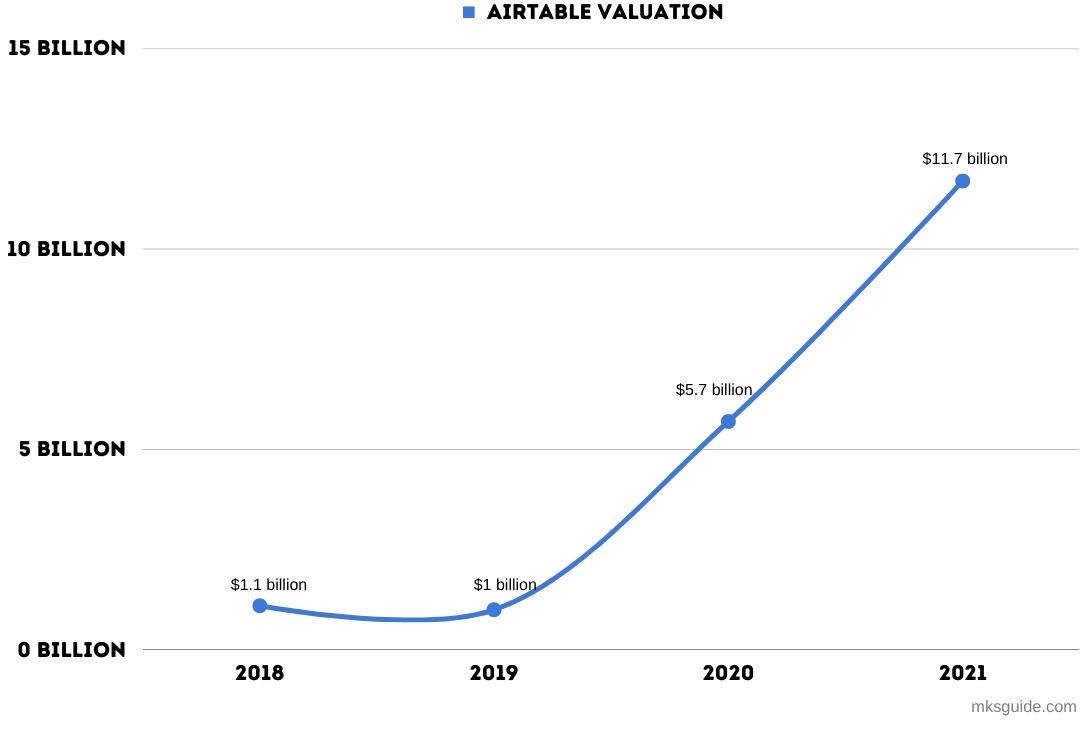
\includegraphics[scale=0.5]{methodologie/Airtable_valuation.png}
    \caption[Geschatte waarde van Airtable]{Geschatte waarde van Airtable van 2018 tot 2021 \autocite{Khemchandani2023}.}
    \label{fig:airtable_value}
\end{figure}

% Stabiel
Airtable heeft de afgelopen twee jaar (januari 2021 tot december 2022) gemiddeld één tot twee incidenten per maand gehad \autocite{AirtableStatus}. Verder werden deze incidenten meestal ook nog de dag zelf opgelost. Het voldoet dus aan de vastgelegde requirements. \\
% https://status.airtable.com/history

% Gebruikersbasis
Airtable wordt gebruikt door meer dan 300.000 bedrijven, waaronder Shopify, Nike en AT\&T. Bovendien gebruikt 80\% van de Fortune 100\footnote{Groep met de 100 grootste bedrijven van de Verenigde Staten} het platform \autocite{Prokopets2022}. Daarnaast heeft meer dan 30\% van de klanten zich ingeschreven voor een betaald plan. Hieruit kan dus afgeleid worden dat het platform een goede gebruikersbasis heeft. \\
% https://nira.com/companies-that-use-airtable/


\section{AppSheet}

% Low-code / Flexibel
De tweede kandidaat voor het onderzoek is het no-code platform Google AppSheet. Het voorziet een groot aantal pasklare templates of 'sample apps' die voor verschillende use cases gebruikt kunnen worden \autocite{AppSheetTemplates}. Alhoewel het platform in het algemeen minder flexibel is dan Podio of Airtable, voldoet het wel aan de requirement. Verder heeft het platform ook een eigen API, maar deze is iets minder uitgebreid dan diegene van Airtable of Podio \autocite{AppSheetAPI}. \\
% https://hawksey.info/blog/2023/03/introducing-appsheetapp-a-google-apps-script-library-helper-class-for-the-appsheet-api/?amp=1

Daarnaast wordt het platform vaak gebruikt door organisaties met meer dan 10.000 werknemers \autocite{Enlyft}. Meta Platforms, Inc.\footnote{https://www.meta.com/} of kortweg Meta, het Amerikaans moederbedrijf van ondere andere facebook, maakt bijvoorbeeld gebruik van AppSheet. Verder is het platform geïntegreerd met Google Workspace en wordt ervan verwacht dat het blijft groeien \autocite{Anand2022}. Bovendien heeft Google Workspace in 2022 aangekondigd dat ze van plan zijn om te investeren in cursussen en opleidingen voor AppSheet. Uit voorgaande informatie kan dus besloten worden dat AppSheet ook een futureproof platform is. \\ 
% https://enlyft.com/tech/products/appsheet
% https://workspace.google.com/blog/product-announcements/hidden-secret-open-secret-year-ahead-appsheet

Vervolgens kan er besloten worden dat AppSheet voldoet aan de stabiliteits-requirement. Sinds begin 2023 heeft het platform nog maar één keer down time gehad, namelijk in januari 2023 \autocite{AppSheetStatus}. \\
% https://www.saashub.com/appsheet-status

Ten slotte zijn ook tal van automatisaties mogelijk via AppSheet. Deze worden in het platform 'bots' genoemd. \autocite{Wong2021}. \\
% https://workspace.google.com/blog/developers-practitioners/what-no-code-automation-looks-appsheet


\section{De uit te bouwen Use Case}

Als use case werd in samenspraak met Quivvy Solutions gekozen voor een eenvoudige applicatie die een simpel stageproces bijhoudt. Ten eerste moet er dus een lijst met studenten en hun gegevens bijgehouden worden. Bovendien moet elke student gelinkt zijn aan een dossier, waar verschillende zaken aan vasthangen zoals onder andere een toegewezen begeleider, sollicitaties die de student gedaan heeft, evaluaties gegeven door een begeleider, een toegewezen stageopdracht en een totaalscore voor het dossier. Hieruit volgt dus dat er ook andere lijsten zoals docenten, sollicitaties,$\ldots$ aanwezig moeten zijn binnen de applicatie. Daarnaast heeft een student ook een richting die dan op zich meerdere specialisaties bevat, dit zijn ook elementen die als lijst moeten worden opgeslagen. Vervolgens moet er ook de mogelijkheid zijn om het dossier eenvoudig om te vormen naar een pdf-bestand. Hiermee is het concept van de use case toegelicht, een verdere uitwerking volgt in de analysefase van het onderzoek. \\

\section{Onderzoek} 

Voor het onderzoek wordt de gekozen use case uitgewerkt, eerst in Podio en daarna in Airtable en AppSheet. Tijdens het uitwerken worden de alternatieven vergeleken met Podio op basis van een set van criteria die hieronder terug te vinden zijn. Telkens als een use case wordt uitgebouwd, wordt ook kort overlopen hoe goed het presteerde op deze criteria. Ten slotte wordt in hoofdstuk \ref{ch:conclusie} een algemene conclusie gegeven. \\

De criteria waarop de alternatieven worden vergeleken zijn als volgt geformuleerd;

\begin{itemize}
    \item Hoe eenvoudig is het om \textbf{relaties} te leggen tussen verschillende onderdelen, bijvoorbeeld tussen een studierichting en zijn specialisaties?
    \item Is het mogelijk om een studentendossier \textbf{automatisch om te vormen} naar een PDF met de nodige informatie? Indien wel, hoe gemakkelijk lukt dit?
    \item Is het mogelijk om via \textbf{workflows} sollicitaties/stageopdrachten aan te maken en deze automatisch te linken met de overeenkomstige student/bedrijf?
    \item Hoe eenvoudig is het om \textbf{calculaties} of berekeningen uit te voeren, zoals een overzicht opstellen van de verschillende stageopdrachten die een bedrijf voorziet?
    \item Hoe aangenaam is de \textbf{gebruikerservaring}? Met name hoeveel keer moet men klikken of navigeren om een bepaald doel te bereiken? Is de tool eenvoudig te gebruiken of is de bediening eerder complex?
    \item Hoe intuïtief is de \textbf{user interface (UI)}? Is deze overzichtelijk of staan er veel zaken door elkaar? Hoe eenvoudig kan een bepaalde functie terug gevonden? Kunnen activiteiten gemakkelijk opgevolgd worden, bijvoorbeeld via dynamische views of tegels?
    \item Hoe \textbf{probleemloos} verloopt het uitbouwen van de use case? Welke problemen komt men allemaal tegen?
\end{itemize}

Aan de hand van deze criteria wordt dus onderzocht of het mogelijk is om de use case uit te bouwen in Airtable of AppSheet en hoe eenvoudig dit lukt.

